% !TEX root = ../paper.tex
\tinysection{Input Definition}
As shown in Figure~\ref{fig:systemoverview}, the input data consists of a finite set of possible instances $\instances=\{\instance_1,\ldots,\instance_n\}$ where each instance $\instance_i$ consists of a set of tuples.
We use the \emph{possible worlds semantics}~\cite{Dalvi:2009:PDD:1538788.1538810} and call $\instances$ as \emph{possible worlds}.
Each world is assigned a probability by the distribution $\possibleworldsdistribution : \instances \to [0,1]$ such that $\sum_i \possibleworldsdistribution(\instance_i) = 1$.
In other words, our input is defined as a discrete probability space $\probabilisticdatabase=(\instances,\possibleworldsdistribution)$.

\tinysection{Goal}
An application theoretically may require scanning through all possible worlds, in order to aggregate the probabilities where the corresponding worlds contain some target \emph{set} of tuples.
In the context of Entity Resolution task, an application may require aggregating probabilities of all predictions that contain tuples labeled by a target $eid$. 
For convenience, we will refer to these aggregated probabilities as \emph{marginal probabilities} or simply \emph{marginals} in the rest of the paper.
Our goal is then to help the application efficiently explore and compute marginals in a practical way without iterating through a large number of possible worlds.

\tinysection{System Overview}
We begin by giving the reader an overview on how the input flows \emph{theoretically} and \emph{practically} to a client-side application.
In Figure~\ref{fig:systemoverview}, the red dashed lines encompasses a theoretical data flow that iterates through all possible worlds.
In practice, possible worlds in the input will converted into an initial form of representation.
Based on the initial form, further compression can be made that provides a materialized view over the input.
The materialized view can be efficiently queried and the query result will be simplified before being presented to the application.

\begin{figure*}[ht!]
    \centering 
     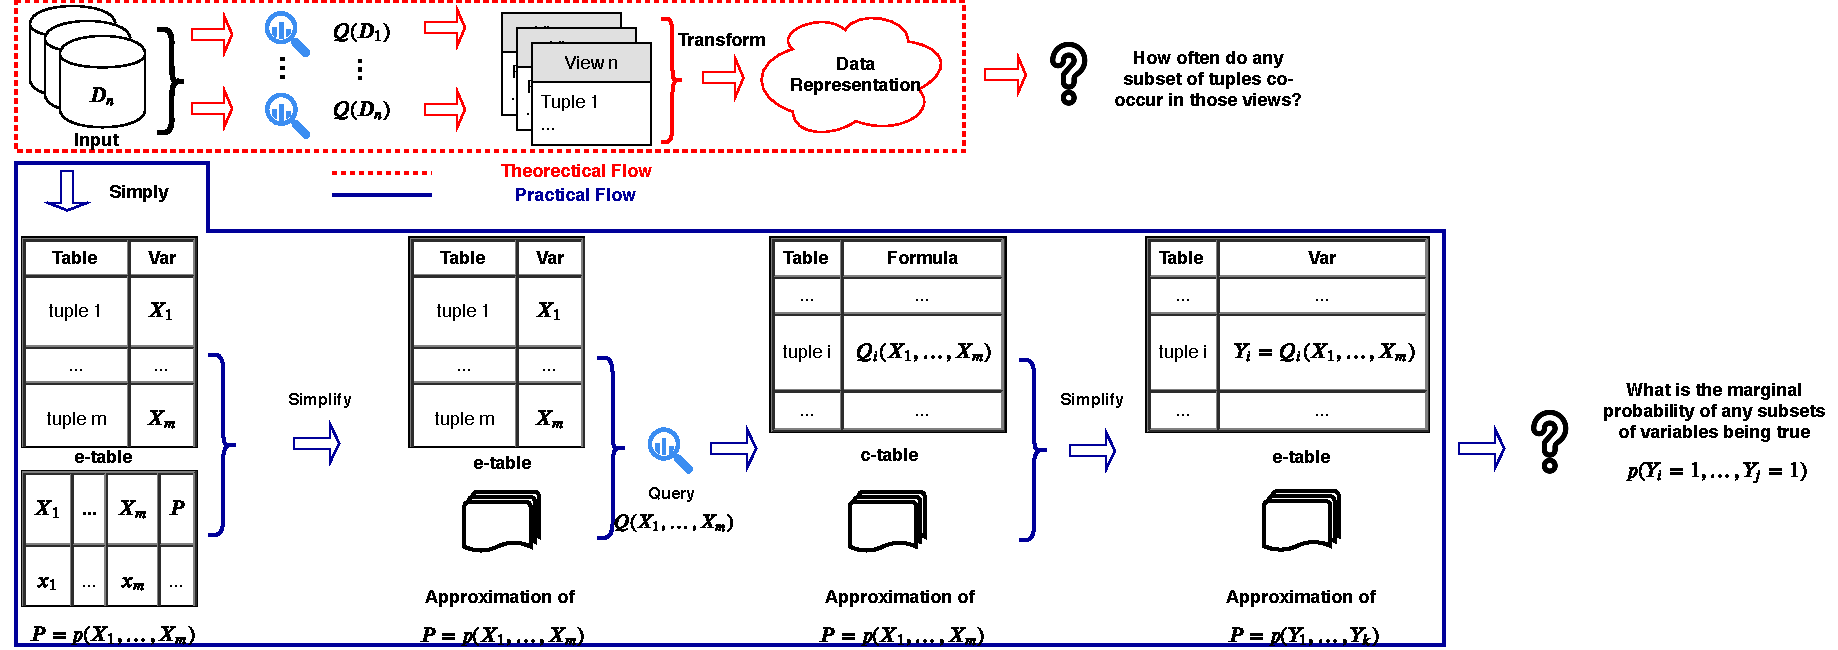
\includegraphics[width=\textwidth]{ProbabilisticDatabaseSummarization/graphics/Data_Flow_Diagram.pdf}
     
 \bfcaption{Theoretical v.s. Practical Data-flows.}
 \label{fig:systemoverview} 
 \trimfigurewhitespace
\end{figure*} 

\subsection{Practical Input Representation}
\label{sec:outputrepresentation}
The previous definition of $\instances$ does not suggest a practical representation, especially when explicit enumeration of all possible worlds is not feasible when $n$ is very large.

\tinysection{C-tables and pc-tables}
We adopt \emph{c-tables} to compactly represent $\instances$. 
A \emph{c-table}~\cite{suciu2009probabilistic} is a set of \emph{distinct} tuples contained in all possible worlds, with each tuple annotated by a propositional formula over random variables.
A \emph{valuation} over these variables assigns each propositional formula a truth value, indicating the existence of the corresponding tuple in a world.
There is a many-to-one mapping from valuations to a possible world.
Extending a c-table by a joint probability distribution over random variables, the resulting \emph{pc-table} can represent any probabilistic database $\probabilisticdatabase$~\cite{suciu2009probabilistic}.

\tinysection{Simplified C-tables}
For our example application, there are two limitations by adopting a general c-table representation.
Firstly, it is difficult to obtain such propositional formula due to lack of knowledge on how tuples are correlated in $\probabilisticdatabase$.
That is, due to complex nature of the function that generates $\probabilisticdatabase$, it is generally hard to formulate how tuples are correlated.
Secondly, the mapping from valuations of variables to possible worlds is many-to-one for a general c-table.
To compute desired marginals, it may require an expensive aggregate over all valuations that map to the same world. 

To overcome the limitations, we represent our input by a family of simplified c-tables, which we call \emph{existence tables} or simply \emph{e-tables}.
Each tuple $\tuplesymbol_i$ in an e-table is annotated with a single random variable $X_i$ whose value is $1$, meaning that the $i$th tuple exists in a world, or $0$ otherwise.
We refer to these variables as \emph{existence variables}.
There is an \emph{one-to-one} mapping from a valuation of existence variables $(x_1,\ldots,x_n)\in\{0,1\}^n$ to a world $\instance$.
The probability of the world (i.e., $\possibleworldsdistribution(\instance)$) can be computed directly from the joint probability distribution $p(X_1=x_1,\ldots,X_n=x_n)$.
When it is clear from context, we abuse notation and denote the distribution $p(X_1=x_1,\ldots,X_n=x_n)$ also as $\possibleworldsdistribution$.
We call an e-table, together with $\possibleworldsdistribution$, a \emph{pe-table}. 

\subsection{Summarizing Joint Distribution}
It is not practical, both in space and marginal computation efficiency, to present pe-table in a view that iterates through all valuations (i.e., worlds) of existence variables.
Hence we need a view that summarizes $\possibleworldsdistribution$ into a more compact form.

\tinysection{Naive Summary}
There can be a set of tuples $\{\ldots,\vec t_i,\ldots\}$ independent of each other such that, 
$$p(\ldots,X_i=1,\ldots)=\Pi_i\;p(X_i=1)$$
In other words, we do not need to store valuations of any combination of those variables in the view, which greatly reduces the number of parameters.
We name the set of parameters $p(X_i=1)$ as a \emph{naive summary} and return to it through out the rest of this paper.
The naive summary is often referred to as \emph{tuple-independent} model~\cite{suciu2009probabilistic}.
When variables are correlated, which is prevalent in our example application, the marginals computed from a naive summary are error-prone.

\tinysection{Loss-less Summary}
For tuples whose variables that are correlated, a \emph{factor graph}~\cite{friedman1999learning} that is equivalent to the marginal probability distribution over these variables, is a sufficient condition for computing any relevant marginals. 
However, it requires heavy weight inference to obtain such set of factors and for each factor, the number of parameters is still exponential to the number of variables that the factor contains.

\tinysection{Lossy Summary}
Practically an application may not require computing exact marginals for \emph{every} set of tuples and we can \emph{cache} marginals that are frequently computed and offer estimation on others. 
Specifically, in our example Entity Resolution task, an application may require to explore labelled tuples that are contained in \emph{all} possible predictions, and tuples that are (in-)frequently or otherwise statistically significant.
The application may tolerate inexact marginal computation for other sets of tuples. 
This observation motivates us to study the option of a \emph{lossy} summary containing only a limited number of marginals and offers estimation on marginals not contained.

\subsection{Pattern-based Summary}

\tinysection{Patterns}
We name a set of co-existing tuples as a \emph{pattern}.
More formally we define a \emph{pattern} as an arbitrary binary vector $\pattern=(x_1,\ldots,x_n)$ with $x_i=1$ meaning the $i$th tuple being present in the pattern.
A pattern $\pattern$ is \emph{contained} in the other $\bar{\pattern}$ if $\forall i, x_i\leq \bar{x}_i$, denoted as $\pattern \subseteq \bar{\pattern}$.
Note that a world $\instance$ is a pattern by definition.
Randomly drawing a world $\instance\in\instances$ from $\probabilisticdatabase$, the probability that it contains pattern $\pattern$ is defined by:
\begin{equation*}
  p(\instances \supseteq \pattern) = \sum_i\possibleworldsdistribution(I_i)\mathbf{1}_{\pattern}(I_i) \;\text{where}\;  \mathbf{1}_{\pattern}(I_i)  =
    \begin{cases}
      1 & \text{if $I_i \supseteq \pattern$}\\
      0 & \text{otherwise}\\
    \end{cases}       
\end{equation*}
In pe-tables, $\marginal$ is equivalent to marginal probability $p(X_1\geq x_1,\ldots,X_n\geq x_n)$.
We call $\marginal$ as the \emph{marginal} of a pattern.

\tinysection{Pattern-based Summary}
Denote the mapping $\encoding_{max}$ from each pattern $\pattern$ to its marginal:
$$\encoding_{max} = \comprehension{\pattern \rightarrow \marginal}{\pattern \in \{0,1\}^n}$$
A \emph{pattern-based summary} $\encoding$ is any such partial mapping $\encoding \subseteq \encoding_{max}$. 
We denote the marginal of pattern $\pattern$ in summary $\encoding$ by $\encoding[\pattern] $ ($= \marginal$).
When it is clear from context, we abuse syntax and also use $\encoding$ to denote the set of patterns it maps (i.e., $domain(\encoding)$).
Hence, $|\encoding|$ is the number of mapped patterns, which we call the summary's \emph{verbosity}.


